% !TEX root = SCCOMP.tex
% This work is licensed under the Creative Commons
% Attribution-NonCommercial-ShareAlike 4.0 International License. To view a copy
% of this license, visit http://creativecommons.org/licenses/by-nc-sa/4.0/ or
% send a letter to Creative Commons, PO Box 1866, Mountain View, CA 94042, USA.

\chapter{Large Sparse Linear Systems}
\section{Modelproblems and discretization}%
\label{sec:Modelproblems and discretization}


\begin{equation}\label{eq:eq_1}
	\frac{\partial^2 u}{\partial x_1^2} + \frac{\partial^2 u}{\partial x_2^2} =: \laplace u = f(x) 
\end{equation}
with $\Omega \subset \R^2$ bounded, open domain and 
$ x =
\begin{pmatrix}
x_1 \\
x_2
\end{pmatrix}
\in \Omega$
\begin{figure}[H]
	\center
\begin{tikzpicture}[scale=3]
		
		\def \xone{0};
		\def \yone{0};		
		% draw coordinate system
		\coordinate (A) at (\xone,\yone);
		
		\draw[->] (A) -- ++(0,1);
		\draw[->] (A) -- ++(1,0);
		\draw[->] (A) ++(0.9,0.5) -- ++(0.5,0);

		% a circle is easier to draw than another object
        \draw (A) ++(0.5,0.5) circle (0.4cm);
        
        \fill[black,font=\footnotesize] (A) ++(1,0) node[below] {$x_{1}$}
										(A) ++(0,1) node[left] {$x_{2}$}
										(A) ++(1.4,0.5) node[below] {$n$};
                                        
\end{tikzpicture}

\caption{example $\Omega$,  $n$   outer normal on $\partial \Omega$}
\label{first picture}
\end{figure}

n outer normal on $\partial \Omega$
with boundary conditions
\[
\alpha u + \beta \frac{\partial u}{\partial n} = g \qquad \text{ on } \partial \Omega
.\] 

If \begin{itemize}
	\item $ \beta = 0$, we get a Dirichlet problem.
	\item $ \alpha \neq 0$, we get a Neumann problem.
	\item $\alpha = 0 \text{ and } \beta = 1$, we have
		\begin{enumerate}
			\item Since $u = \text{const}$ solves \href{eq:eq_1}{(1)} % TODO FIX THIS
				for $f=0 \text{ and } g = 0$, the solution to \href{eq:eq_1}{(1)} is unique up to a constant
			\item Integrating \href{eq:eq_1}{(1)} over $\Omega$ and Green's formula yield
				\[
				- \int_{\partial\Omega} \frac{\partial u}{\partial n} = - \int_{\Omega} \laplace u = \int_{\Omega} f
				.\] 
				This means, we get a compatibility condition
				\[
				\int_{\partial \Omega} g + \int_{\Omega}f = 0
				.\] 
		\end{enumerate}
\end{itemize} 

Another variant of \href{eq:eq_1}{(1)} is
\[
	Lu := \nabla(A\nabla u)
.\] 
where A is a positive definite matrix.

\begin{equation}
	\label{eq_2}
LU = f \qquad \in \Omega \text{ + boundary condition}
\end{equation}

\section{Discretization with finite differences}%
\label{sec:Discretization with finite differences}

The basic idea is

%TODO Hier kommt noch etwas Inhalt für den ich nicht schnell genug war.


\begin{itemize}
	\item \underline{(1D-case):} 
		%Das fehlt auch alles
	\item \underline{(2D \& 3D cases):} 
		The laplacian is the sum of all second derivatives
		\[
			\laplace = \partial x_1^2 + \partial x_2^2 (+\partial x_3^2)
		.\] 
		With (possibly) different step width $h$ in each coordinate direction we get
		\begin{align*}
			\laplace u(x) &= \frac{u(x_1 + h_1, x_2) - 2u(x_1, x_2) + u(x_1 -h_1, x_2)}{h_1^2}\\
						  &+ \frac{u(x_1, x_2 + h_2) - 2u(x_1, x_2) + u(x_1, x_2 -h_2)}{h_2^2}
		\end{align*}
		but for $h_1 = h_2 = h$ we get
		\[
			\laplace u(x) \approx \frac{1}{h^2}\left[u(x_1+ h, x_2) + u(x_1-h, x_2) + u(x_1, x_2 -h) + u(x_1, x_2 -h) -4u(x_1, x_2)\right]
		.\] 
		Denoting the forward/backward difference formulas
		in the direction i by $\delta_{i}^{+}$ and $\delta_{i}^{-}$ we can write
		\[
			\laplace u(x) \approx \sum_{i=1}^{2}{\delta_{i}^{+}\delta_{i}^{-}u(x)}=:\laplace_{h}^{(5)}u(x)
		.\] 
		The formula can be sketched as a stencil, the so called " 5-point stencil "
		%\tikzset
{
	treenode/.style = {circle, draw=black!60, fill=white!40, very thick, minimum size=6mm}
}

\begin{figure}[H]
	\center

	\begin{tikzpicture}%[level/.style={sibling distance = 2cm/#1, level distance = 3cm}]
	
	\def \xone{0};
	\def \yone{0};
	
	\coordinate (root) at (\xone ,\yone);
	\draw (root) ++ (-1,0) -- ++(2,0);
	\draw (root) ++ (0,-1) -- ++(0,2);

	%draw nodes
	\node [treenode] at (root) {-4};
	\node [treenode] at (root) ++ (-1,0) {1};
	\node [treenode] at (root) ++ (1,0) {1};
	\node [treenode] at (root) ++ (0,1) {1};
	\node [treenode] at (root) ++ (0,-1) {1};

		
	\end{tikzpicture}
	
\caption{5-point stencil (second order accurate)}
\label{five_point}
\end{figure}

		where the values in the nodes correspond to the coefficients in the formula.
		Other possible stencils are:
		\begin{itemize}
			\item 5-point-stencil, $2^{\text{nd}}$ order accurate
				%\begin{figure}[H]
	\center

	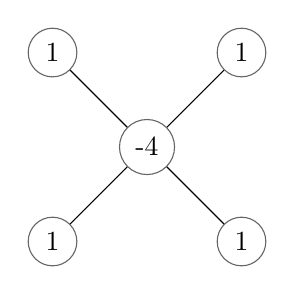
\begin{tikzpicture}

	\def \xone{0};
	\def \yone{0};
	\def \h{1.2}	

	\coordinate (M) at (\xone ,\yone);
	\coordinate (LU) at (\xone-\h ,\yone-\h);
	\coordinate (RU) at (\xone+\h ,\yone-\h);
	\coordinate (LO) at (\xone-\h ,\yone+\h);
	\coordinate (RO) at (\xone+\h ,\yone+\h);
	\draw (LU) -- (RO);
	\draw (RU) -- (LO);

	%draw nodes
	\node[circle,draw=black!60, fill=white!40] at (M) {-4};
	\node[circle,draw=black!60, fill=white!40] at (LO) {1};
	\node[circle,draw=black!60, fill=white!40] at (RO) {1};
	\node[circle,draw=black!60, fill=white!40] at (LU) {1};
	\node[circle,draw=black!60, fill=white!40] at (RU) {1};

		
	\end{tikzpicture}
\caption{rotated 5-point stencil}
\label{five_point_rot}
	
\end{figure}

			\item 9-point-stencil,  $2^{\text{nd}}$ order accurate and even $6^{\text{th}}$ order accurate for harmonic funtions
				%\begin{figure}[H]
	\center

	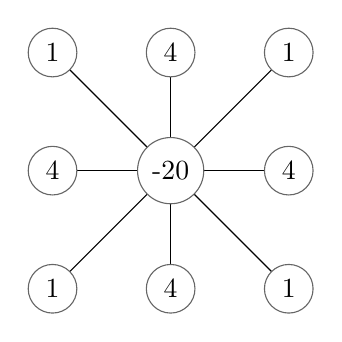
\begin{tikzpicture}
	
	\def \xone{0};
	\def \yone{0};
	\def \h{1.5}	

	\coordinate (M) at (\xone ,\yone);
	\coordinate (L) at (\xone-\h ,\yone);
	\coordinate (R) at (\xone+\h ,\yone);
	\coordinate (O) at (\xone ,\yone+\h);
	\coordinate (LU) at (\xone-\h ,\yone-\h);
	\coordinate (RU) at (\xone+\h ,\yone-\h);
	\coordinate (LO) at (\xone-\h ,\yone+\h);
	\coordinate (RO) at (\xone+\h ,\yone+\h);
	\coordinate (U) at (\xone ,\yone-\h);

	\draw (L) -- (R);
	\draw (U) -- (O);
	\draw (LU) -- (RO);
	\draw (RU) -- (LO);

	%draw nodes
	\node[circle,draw=black!60, fill=white!40] at (M) {-20};
	\node[circle,draw=black!60, fill=white!40] at (L) {4};
	\node[circle,draw=black!60, fill=white!40] at (R) {4};
	\node[circle,draw=black!60, fill=white!40] at (O) {4};
	\node[circle,draw=black!60, fill=white!40] at (U) {4};

	%draw diagonal nodes
	\node[circle,draw=black!60, fill=white!40] at (LO) {1};
	\node[circle,draw=black!60, fill=white!40] at (RO) {1};
	\node[circle,draw=black!60, fill=white!40] at (LU) {1};
	\node[circle,draw=black!60, fill=white!40] at (RU) {1};

	
	\end{tikzpicture}
	\caption{9-point stencil}
\label{nine_point}
	
\end{figure}

		\end{itemize}
\end{itemize}

\section{Finite difference on a grid}%
\label{sec:Finite difference on a grid}
Let $\Omega =(0, X_{E}) \times (0,Y_{E})$ and subdivide each interval into $N_{x}+1 / N_{y} + 1$ subintervals.
\begin{figure}[H]
	\center
\begin{tikzpicture}[scale=3]
		
		\def \xone{0};
		\def \yone{0};		
		% draw coordinate system
		\coordinate (A) at (\xone,\yone);
		
		\draw[\to] (A) -- ++(0,1);
		\draw[\to] (A) -- ++(1,0);
		\draw (A) ++(0.5,0) -- ++ (0,1);
		\draw (A) ++(1,0) -- ++ (0,1) -- ++(-1,0);
		\draw (A) ++(0,0.333) -- ++ (1,0);
		\draw (A) ++(0,0.666) -- ++ (1,0);
		\draw[red!60] (A) -- (A) ++ (0,0.333);
		\draw[blue!60] (A) -- (A) ++ (0.5,0);

        \fill[black,font=\footnotesize] (A)  ++(1,0) node[under] {$x_{E}$}
										(A)  ++(0,1) node[left] {$y_{E}$}
										(A)  ++(0.25,0) node[under] {$h_{x}$}
										(A)  ++(0,0.1666) node[left] {$h_{y}$};
                                        
\end{tikzpicture}

\caption{Visualization of Grid}
\label{example_grid}
\end{figure}

Each node (vertex) in this grid is assigned an index tuple
\[
	(x,y) = (ih_{x}, jh_{y}) = (i,j)
.\] 
for $i \in$





